\documentclass[11pt]{article}
\usepackage{fancyhdr, extramarks, amsmath, amsthm, amsfonts, tikz, algpseudocode, graphicx, tcolorbox}
\usepackage[plain]{algorithm}
\graphicspath {{graphs/}}
\usetikzlibrary{automata,positioning}

\topmargin=-0.45in
\evensidemargin=0in
\oddsidemargin=0in
\textwidth=6.5in
\textheight=9.0in
\headsep=0.25in
\title{\textbf{Introduction to Artificial Intelligence\\
		\large Project 1: Maze on Fire}}
\author{Brenton Bongcaron and Abe Vitangcol\\NetIDs: bdb101 and alv88}
\date{February 19, 2021}
\begin{document}
	\maketitle
	\pagebreak
\section{No Maze is the Same: Creating Mazes}
The premise of the project is an agent being trapped in a maze. They start at the top left of the maze and need to get to the very bottom right of the maze. To create the maze environment, we created a function called buildMaze within maze.py which makes the maze in the form of a matrix.
\begin{verbatim}
def buildMaze(dim, p, firep=0):
    maze = [ [1 for col in range(dim)] for row in range(dim) ]
    # Randomly arranges obstacles
    fireTile = False
    for i in range(dim):
        for j in range(dim):
            rand = random()
            if rand <= p:
                maze[i][j] = 0
    # Randomly selects a fire tile
    while True:
        randx = randrange(dim)
        randy = randrange(dim)
        if maze[randx][randy] == 1 and randx != 0 and randx != (dim - 1)
        and randy != 0 and randy != (dim - 1):
            maze[randx][randy] = 2
            break
    # Ensure Start and Goal spaces are empty
    maze[0][0] = 1
    maze[dim - 1][dim - 1] = 1
    return maze

\end{verbatim}
Building the maze needs only a few requirements: the size of the maze (dim), and the obstacle density of the maze (p). The obstacle density is between 0 and 1, exclusive, and our code is ready to output an error message should a value be inputed outside that range. The maze is generated as a matrix with all of its entries, from (0,0) to (dim - 1, dim - 1), are 1. Then, going through each tile one by one using a nested for loop, we used random() as a way to randomize the maze, and if the value obtained from random() was less than or equal to the obstacle density, it became the obstacle, which means the value of the matrix at that coordinate was 0. When it finishes going through all of the tiles of the maze, we need to make sure that (0,0) and (dim - 1, dim - 1) are not obstacles, as they serve as the start and goal spaces, respectfully. So, we simply force these two spaces to be 1 (non-obstacle spaces) so the agent can be loaded in and is able to walk on top of the goal space.
The other part of this code is for the fire, which simply picks a random location on the maze and designates this as the fire, making that part of the matrix equal to 2. If the space is a fire, then the maze at that point will equal two. Like the obstacles, if it was created on the start or goal spaces, it will be overwritten for a non-obstacle space.
	\pagebreak
\section{Finding the path to the goal: DFS}
For the first search algorithm, we were tasked at creating a Depth First Search algorithm and use it to help the agent navigate through the maze. To help us with creating this algorithm, we defined a helper function that says whether a move is valid or not, which we can use for both the DFS function as well as future functions too.
\begin{verbatim}
def isValid(maze, coordinate):
    if coordinate[0] < 0 or coordinate[0] >= len(maze) or
       coordinate[1] < 0 or coordinate[1] >= len(maze):
        return False
    if maze[coordinate[0]][coordinate[1]] == 1:
        return True
    return False
\end{verbatim}
Simply called isValid, located within maze.py, it takes in the current maze layout and the coordinate of interest. If the coordinate takes the agent out of bounds of the maze, then it returns false. If the coordinate of the maze is a free space, meaning the coordinate at that matrix location equals 1, then it returns true. There is a third false for fire scenarios, as the second if statement will be skipped as the fire tile is resembled as a 2 on the matrix, not a 1.

Using this, we created the DFS algorithm in maze.py and named it DFS.
\begin{verbatim}
def DFS(maze,start=(0,0),spacesTraveled=[], target=None):
    fringe = [start]
    visited = []
    for alreadyVisited in spacesTraveled:
        visited.append(alreadyVisited)
    prev = {start : None}
    if target is None:
        target = (len(maze) - 1, len(maze) - 1)
    start_time = time.time()
    while fringe:
        (currentRow, currentCol) = fringe.pop()
        ######################################
        # Check the children of currentState #
        ######################################
        if (currentRow, currentCol) == target:
            end_time = time.time()
            elapsed_time = end_time - start_time
            #print(str(elapsed_time) + "s to find path with DFS")
            return prev
        #upChild
        if isValid(maze, (currentRow - 1, currentCol)) and 
        (currentRow - 1, currentCol) not in visited:
            fringe.append((currentRow - 1, currentCol))
            prev.update({(currentRow - 1, currentCol) : (currentRow, currentCol)})
        #leftChild
        if isValid(maze, (currentRow, currentCol - 1)) and 
        (currentRow, currentCol - 1) not in visited:
            fringe.append((currentRow, currentCol - 1))
            prev.update({(currentRow, currentCol - 1) : (currentRow, currentCol)})
        #downChild
        if isValid(maze, (currentRow + 1, currentCol)) and 
        (currentRow + 1, currentCol) not in visited:
            fringe.append((currentRow + 1, currentCol))
            prev.update({(currentRow + 1, currentCol) : (currentRow, currentCol)})
        #rightChild
        if isValid(maze, (currentRow, currentCol + 1)) and 
        (currentRow, currentCol + 1) not in visited:
            fringe.append((currentRow, currentCol + 1))
            prev.update({(currentRow, currentCol + 1) : (currentRow, currentCol)})
        #########################################################################
        # Order (up,left,down,right) chosen so that any moves to the right or   #
        # down (closer to the Goal space, assuming no obstructions) are         # 
        # placed at the top of the stack and popped off before any moves up or  #
        # left.                                                                 #
        #########################################################################
        visited.append((currentRow, currentCol))
    return None
\end{verbatim}
This DFS algorithm requires the current layout of the maze, which is given as the parameter maze. The other three variables are default variables in which if a value is not specified upon calling the DFS function, it simply sets the start as (0,0), the target as nothing, and an empty list for the spacesTraveled. For the start and target, this is for any scenario in which the start and goal are not the typical (0,0) and (dim - 1, dim - 1), allowing flexibility for randomized spaces, if we want to. The spacesTraveled default variable is there for when the fire starts to spread and helps to with visualization when we run simulate.py or render.py.
The DFS algorithm examines the neighbors of the agent's node, with the agent's node called (currentRow, currentCol) in our code. The algorithm starts by pushing the current position of the agent into the stack, then later pops it, examining the popped node and seeing if the space is the goal. If so, it reports the time (currently commented out to save space in our command prompt) and returns the list of nodes the agent traveled through. If the popped node is not the goal space (always not so long as the dim value is greater than 1, which it always is), then it starts to check valid neighbors. It checks the north neighbor (called up child in our comments), the west neighbor (called left child), next the south neighbor (called down child), and finally the east neighbor (called the right child). They are pushed into the stack in this specific order as to prioritize going towards the goal (going either down or right) upon popping the next node. It constantly repeats this until it either has exhausted all nodes and hasn't gotten to the goal or until it reaches the goal.

Figure \ref{DFS_p_vs_successRate} shows a graph of the obstacle density vs the probability that S can be reached from G using our DFS algorithm and a maze size of $dim = 125$, with 100 unique maze runs being performed at each obstacle density, which increases by an interval of 0.2 after each set of 100 tests.

\begin{figure}[h]
\centering
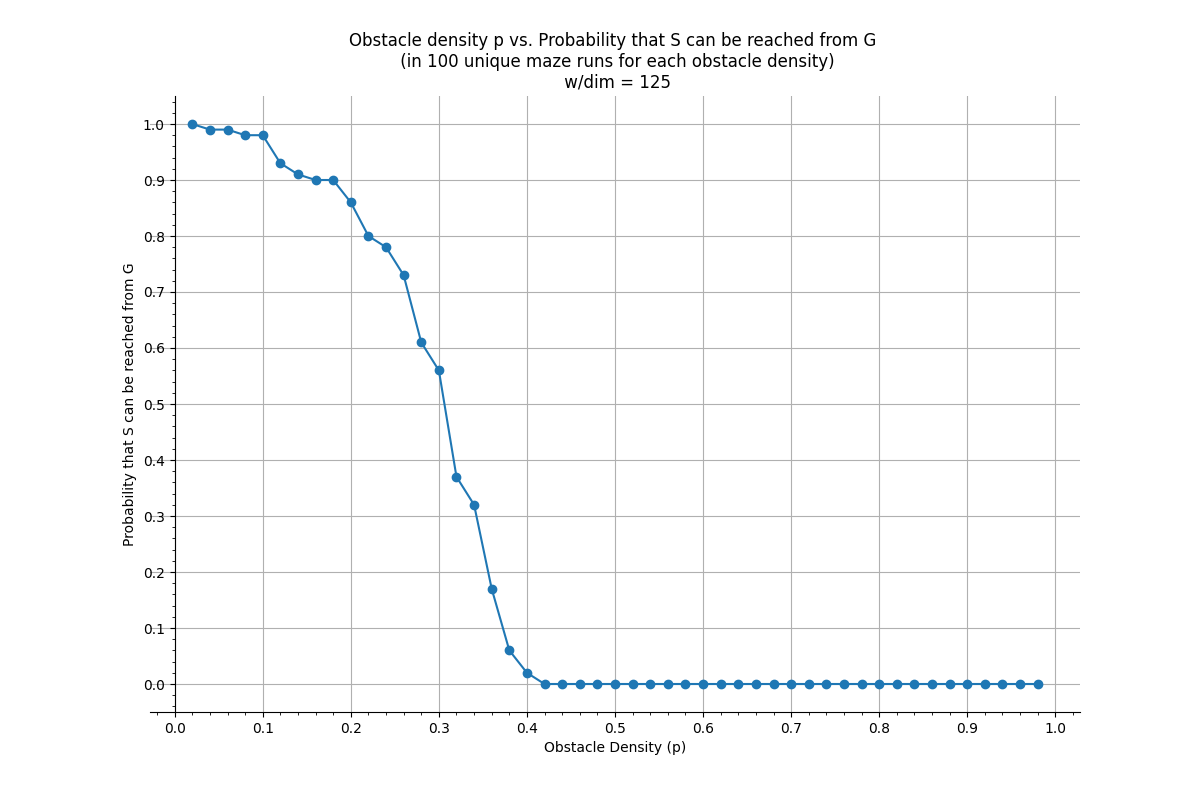
\includegraphics[scale=0.55]{graphs/DFS_obstacleDensity_vs_successRate.PNG}
\caption{A plot of 'obstacle density $p$' vs 'probability that $S$ can be reached from $G$'.}
\label{DFS_p_vs_successRate}
\end{figure}

While a Breadth First Search (BFS) will find an optimal path in getting to the goal (assuming a path to the goal exists), DFS is actually better in a situation like this simply because we already know where the goal is from the start. By simply knowing where the goal is at the beginning of the run, we can simply beeline over to that destination by going down one whole branch to find the goal instead of going through all of the layers of a BFS tree just to eventually see the goal at the end of one of the branches. Simply put, using DFS in this maze is faster than BFS as BFS is always going a worst-case scenario in having to check majority of the nodes to find the goal, sometimes taking about 20 times longer than DFS. If the goal was randomized each run, then BFS would be a better pick as the goal would be somewhere in the middle of its tree rather than at the bottom while DFS would have to search entire branches one at a time to find the goal node somewhere in the middle.
	\pagebreak
\section{BFS and A* Implementation}
After completing the DFS search algorithm, it acted as a skeleton for other search algorithms, like BFS and A*, simply because all of them go through the same process, but they just have a different fringe or organizational method to proceed through the maze.
Both BFS and A* take in the same parameters as DFS, minus some unnecessary parameters such as the target or spacedTraveled. And they work relatively similarly to DFS.

\begin{verbatim}
def BFS(maze, start=(0,0), spacesTraveled=[]):
    fringe = [start]
    visited = []
    for alreadyVisited in spacesTraveled:
        visited.append(alreadyVisited)
    prev = {start : None}
    nodesExplored = 0
    start_time = time.time()
    while fringe:
        (currentRow, currentCol) = fringe.pop(0)
        nodesExplored += 1
        #takes off the first position coordinate off of fringe, acts as dequeue.
        #####################################
        # Checks the condition of the child #
        #####################################
        if (currentRow, currentCol) == (len(maze) - 1, len(maze) - 1):
            end_time = time.time()
            elapsed_time = end_time - start_time
            #print(str(elapsed_time) + "s to find path with DFS")
            return prev, nodesExplored
        #rightChild
        if isValid(maze, (currentRow, currentCol + 1)) and 
        ((currentRow, currentCol + 1) not in visited and 
        (currentRow, currentCol + 1) not in fringe):
            fringe.append((currentRow, currentCol + 1))
            prev.update({(currentRow, currentCol + 1) : (currentRow, currentCol)})
        #downChild
        if isValid(maze, (currentRow + 1, currentCol)) and 
        ((currentRow + 1, currentCol) not in visited and 
        (currentRow + 1, currentCol) not in fringe):
            fringe.append((currentRow + 1, currentCol))
            prev.update({(currentRow + 1, currentCol) : (currentRow, currentCol)})
        #leftChild
        if isValid(maze, (currentRow, currentCol - 1)) and 
        ((currentRow, currentCol - 1) not in visited and 
        (currentRow, currentCol - 1) not in fringe):
            fringe.append((currentRow, currentCol - 1))
            prev.update({(currentRow, currentCol - 1) : (currentRow, currentCol)})
        #upChild
        if isValid(maze, (currentRow - 1, currentCol)) and 
        ((currentRow - 1, currentCol) not in visited and 
        (currentRow - 1, currentCol) not in fringe):
            fringe.append((currentRow - 1, currentCol))
            prev.update({(currentRow - 1, currentCol) : (currentRow, currentCol)})
        #########################################################################
        # Order is (right, down, left, up), the reverse of the DFS. Chosen so   #
        # upon dequeuing (in this case fringe.pop(0)), it will prioritize going #
        # towards the goal per layer of the search before looking left or up.   #
        #########################################################################
        visited.append((currentRow, currentCol))
    return None, nodesExplored
\end{verbatim}

As seen here, the BFS code has a similar structure to DFS. The main difference is how the fringe is used. In DFS, the fringe acted as a stack, having the nodes being pushed in and popped. In BFS, the fringe acts as a queue. When a node is popped (doing fringe.pop(0) is the same as dequeueing), it is checked to see if it is the goal node or not. If so, it does what DFS does with little changes. If not, it checks the node's neighbors. In terms of the priority of searching its neighbors, it does right, then down, then left, then up, appending each one after checking if it's valid. It constantly repeats appending and popping(0) the fringe until it finds the goal, which takes significantly more time than DFS, even if it finds the most optimal path to the goal.

\begin{verbatim}
def aStar(maze, start=(0,0)):
    fringeNodes = [start]
    distances = [0]
    visited = []
    prev = {start: None}
    nodesExplored = 0
    start_time = time.time()
    while fringeNodes:
        # Find the node which has the lowest distance to the goal
        lowestDistance = min(distances)
        index = distances.index(lowestDistance)
        (currentRow, currentCol) = fringeNodes.pop(index)
        ####################### Visualize node just popped from fringe
        distances.pop(index)
        #######################
        nodesExplored += 1
        #####################################################################
        # Check the current condition of the child. If it's the goal, done. #
        # If not, find more children.                                       #
        #####################################################################
        if (currentRow, currentCol) == (len(maze) - 1, len(maze) - 1):
            end_time = time.time()
            elapsed_time = end_time - start_time
            return prev, nodesExplored
        # rightChild
        if isValid(maze, (currentRow, currentCol + 1)) and 
        ((currentRow, currentCol + 1) not in visited and 
        (currentRow, currentCol + 1) not in fringeNodes):
            x_squared = pow((len(maze) - 1) - (currentCol + 1), 2)
            y_squared = pow((len(maze) - 1) - (currentRow), 2)
            nodeDistance = math.sqrt(x_squared + y_squared)
            fringeNodes.append((currentRow, currentCol + 1))
            distances.append(nodeDistance)
            prev.update({(currentRow, currentCol + 1): (currentRow, currentCol)})
        # downChild
        if isValid(maze, (currentRow + 1, currentCol)) and 
        ((currentRow + 1, currentCol) not in visited and 
        (currentRow + 1, currentCol) not in fringeNodes):
            x_squared = pow((len(maze) - 1) - (currentCol), 2)
            y_squared = pow((len(maze) - 1) - (currentRow + 1), 2)
            nodeDistance = math.sqrt(x_squared + y_squared)
            fringeNodes.append((currentRow + 1, currentCol))
            distances.append(nodeDistance)
            prev.update({(currentRow + 1, currentCol): (currentRow, currentCol)})
        # leftChild
        if isValid(maze, (currentRow, currentCol - 1)) and 
        ((currentRow, currentCol - 1) not in visited and 
        (currentRow, currentCol - 1) not in fringeNodes):
            x_squared = pow((len(maze) - 1) - (currentCol - 1), 2)
            y_squared = pow((len(maze) - 1) - (currentRow), 2)
            nodeDistance = math.sqrt(x_squared + y_squared)
            fringeNodes.append((currentRow, currentCol - 1))
            distances.append(nodeDistance)
            prev.update({(currentRow, currentCol - 1): (currentRow, currentCol)})
        # upChild
        if isValid(maze, (currentRow - 1, currentCol)) and 
        ((currentRow - 1, currentCol) not in visited and 
        (currentRow - 1, currentCol) not in fringeNodes):
            x_squared = pow((len(maze) - 1) - (currentCol), 2)
            y_squared = pow((len(maze) - 1) - (currentRow - 1), 2)
            nodeDistance = math.sqrt(x_squared + y_squared)
            fringeNodes.append((currentRow - 1, currentCol))
            distances.append(nodeDistance)
            prev.update({(currentRow - 1, currentCol): (currentRow, currentCol)})
        visited.append((currentRow, currentCol))
    return None, nodesExplored
\end{verbatim}

The A* code (called aStar cause function declaration doesn't like asterisks) still maintains the structure of DFS. Like BFS, A*'s fringe performs differently as now it acts as a priority queue instead of a queue or a stack. Unlike the other two search algorithms, A* includes another array that records the cost and helps with doing priority queue actions. At first, when A* is called, it has a cost of 0 in distances (the helper priority queue) and the start node in the fringeNodes. A* finds the minimum in distances (done by doing min(distances)) and stores that value in the variable name lowestDistance. Next, we find the index at which this lowestDistance occurs in distances (by doing distances.index(lowestDistance)) and store that information in a variable called index. After obtaining the index of the lowest cost, we pop both priority queues at that index, with the value from fringeNodes being stored as (currentRow, currentCol) and the value from distances simply being lost.
Now that a node has been obtained, it goes through the same procedure as BFS and DFS, where it checks if the current node is the goal or not, reporting similar things should it be the goal node. When it checks for its neighbors, order doesn't technically matter, but we have it set to the same order as BFS. To calculate the distances, we simply use euclidean distance from the node in question (the right / left / down / up child) to the goal and record it in a variable called nodeDistance. Once calculated, we append the node in question to fringeNodes and append nodeDistance to distances at the same time in order to keep both of these items at the same index. After checking all the valid neighbors, A* goes back to the top and finds the minimum distance, finds its index, pops both the node at that index in fringeNodes and in distances, and goes back to checking neighbors again. This repeats until it reaches the goal and take much less time than BFS, although it does explore more nodes than it. 

Figure \ref{BFS-A} depicts the average number of nodes explored by BFS - number of nodes explored by A\text{*} vs obstacle density p at a size of \texttt{dim = 100}.

\begin{figure}[h]
\centering
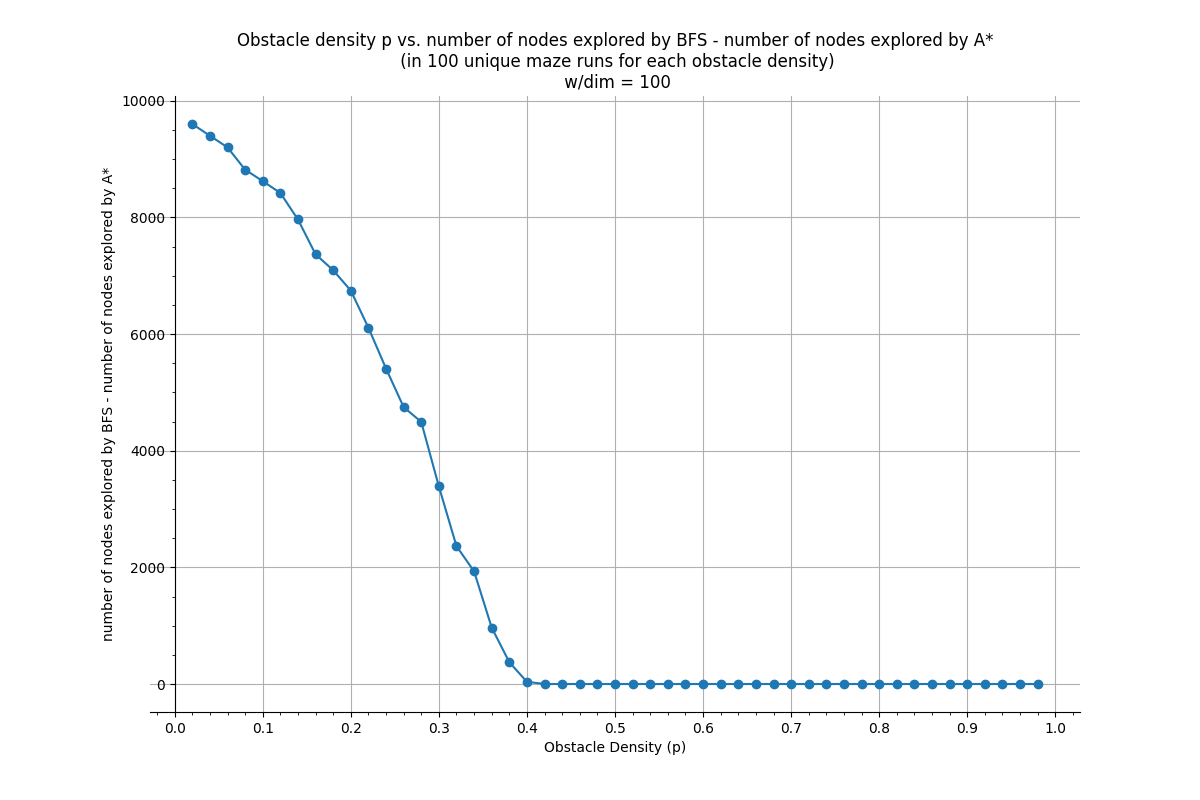
\includegraphics[scale=0.55]{graphs/obstacleDensity_vs_nodesBFSminusNodesAstar.PNG}
\caption{A plot of 'obstacle density $p$' vs '\# nodes explored by BFS - \# nodes explored by A*'.}
\label{BFS-A}
\end{figure}

Take note that if a maze was considered to be impossible, it was still recorded in the data, but now the nodes explored will be 0 as it technically hasn't moved from the start.
	\pagebreak
\section{Time is Everything}
The machine used for testing the maximum dimension of a maze that can be solved with DFS, BFS, and A* had the following specs:
\begin{itemize}
\item Intel(R) Core(TM) i7-4600M @2.90GHz
\item 8.00 GB RAM
\end{itemize}
The maximum dimension maze that could be solved in $<1$ min using DFS was 504 by 504.\\\\
The maximum dimension maze that could be solved in $<1$ min using A* was 511 by 511.\\

Since BFS clearly was going to reach a 1 minute time at a smaller dimension than DFS and A* and BFS notably explores more nodes layer by layer rather than probing a specific branch of children, we thought it would be worthwhile to explore the relationship between the dimension of the maze to be BFS'ed and the time elapsed to find the path to the goal.\\

\begin{figure}[h]
\centering
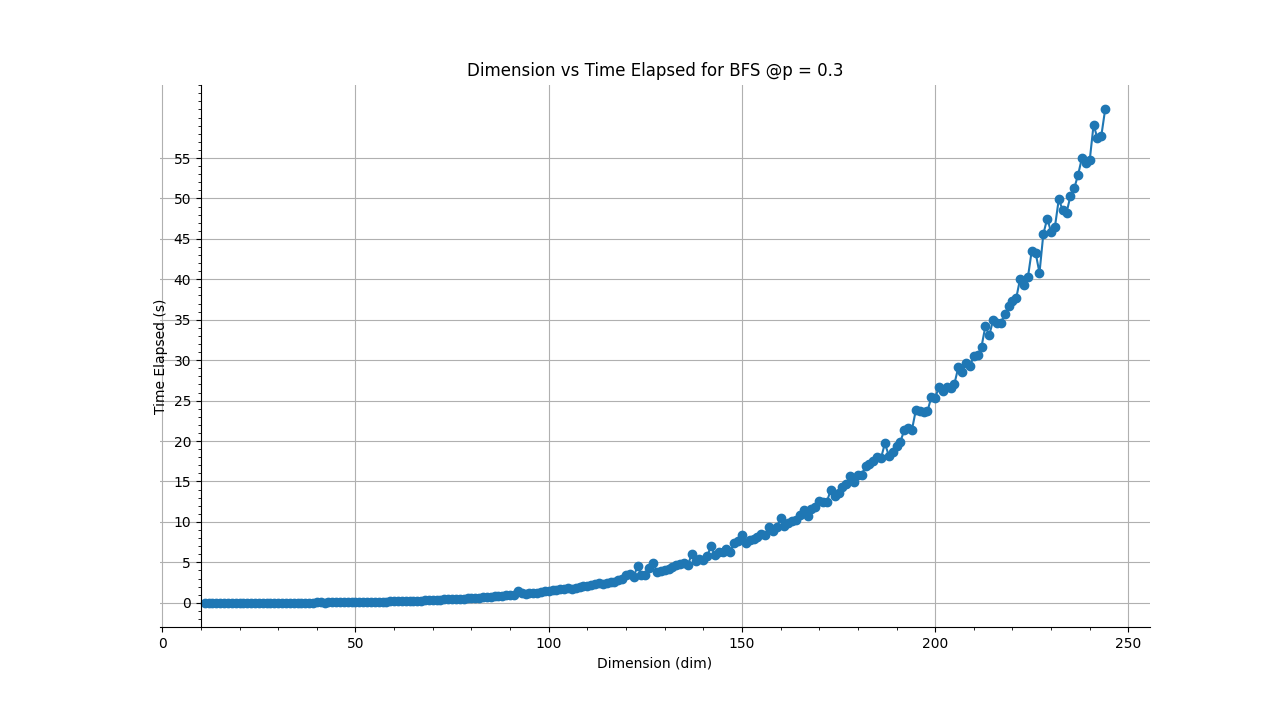
\includegraphics[scale=0.5]{dimVStimeBFS_MAX243.PNG}
\caption{A plot of maze dimension vs. time elapsed in seconds to find the goal with BFS}
\label{BFStime}
\end{figure}
The time it takes to find a path using BFS increases exponentially with respect to the dimension of the maze.

Plots were not generated for DFS and A* because the time elapsed to find the goal with these two algorithms is heavily dependent on probability and because of our program freezing upon trying to create a new maze when the original maze doesn't have a path for either the fire or the agent to get to the goal, especially at higher sizes. With DFS, the less the algorithm has to put children in the north or west directions into the fringe, the shorter the time it takes to find a path to the goal. With A*, the less the algorithm has to put children that are further away from the top left to bottom right diagonal into the fringe, the shorter the time it takes to find a path to the goal.
	\pagebreak
\section{This Maze is on Fi-yah: A New Strategy}
After completing the code for A* and BFS, now it is time to make things a bit more chaotic: set the maze on fire. Previously, there was code regarding the maze being on fire which was previously been brushed off to the side as we were not testing those scenarios yet. Now they become a bit more relevant.
While we have discussed how, upon building the maze, the fire location is randomly selected, one of the next algorithms needed to accurately simulate this burning maze is having the fire spread, which we named fireSpread within maze.py.

\begin{verbatim}
def fireSpread(maze, fireProbability):
    newMaze = copy.deepcopy(maze)
    newFires = []
    for currentRow in range(len(maze)):
        for currentCol in range(len(maze)):
            if isValid(maze, (currentRow, currentCol)) and (currentRow, currentCol) not in newFires:
                k = 0
                if isBurning(maze, (currentRow - 1, currentCol)):
                    k += 1
                if isBurning(maze, (currentRow, currentCol - 1)):
                    k += 1
                if isBurning(maze, (currentRow + 1, currentCol)):
                    k += 1
                if isBurning(maze, (currentRow, currentCol + 1)):
                    k += 1
                fireProb = 1 - pow((1 - fireProbability),k)
                if random() <= fireProb:
                   newMaze[currentRow][currentCol] = 2
                   newFires.append((currentRow, currentCol))
    return newMaze, newFires
\end{verbatim}

This algorithm takes the current layout of the maze and returns a new layout of the maze where fire spread onto free tiles (any tile represented in the matrix as 1), which is why the maze parameter is necessary. The parameter fireProbability dictates how easily the fire will spread onto its neighbors, between 0 and 1 exclusive. The higher the probability, the higher chance the fire will spread onto its neighbors. To calculate the chance of the fire spreading, we use the formula $1 - (1 - fireProbability)^k)$, where k represents the number of fire tiles neighboring a free tile. After performing random(), if random was less than this calculated number, that free tile turned into fire.

With the declaration of a new type of tile comes the need to have another function to help our lost agent to get out safely. As such, we decided to use the same logic as isValid and made another function called isBurning.

\begin{verbatim}
def isBurning(maze, coordinate):
        if coordinate[0] < 0 or coordinate[0] >= len(maze) or coordinate[1] < 0 or coordinate[1] >= len(maze):
            return False
        if maze[coordinate[0]][coordinate[1]] == 2:
            return True
        return False
\end{verbatim}

While it looks like it would perform similar to isValid and doesn't seem necessary, we thought this would be useful in thinking about strategies in having our agent navigate through the maze, especially since we see fires as more dangerous than a wall. Both of us knew one thing: we wanted to utilize this isBurning to add a cost factor to an agent's moves and pick the one that had the least cost. As such, we made a copy of the aStar function and created a version that considered the costs, called aStarPlus. It is almost the same as aStar, but there are various differences to help it navigate better.

\begin{verbatim}
    def checkCost(maze, checkNode, direction, firep, spacesTraveled):
    # A helper function to help make any node being checked if it's dangerous \\
    # or not by adding more cost based on if it has a fire nearby \\
    # or wall nearby.
        addedCost = 0
        if direction == "right":
            if (checkNode[0], checkNode[1]) in spacesTraveled:
                addedCost += 1
            addedCost += calcCost(maze, (checkNode[0], checkNode[1] + 1), firep)
            addedCost += calcCost(maze, (checkNode[0], checkNode[1] + 2), firep)
            addedCost += calcCost(maze, (checkNode[0] + 1, checkNode[1] + 1), firep)
            addedCost += calcCost(maze, (checkNode[0] - 1, checkNode[1] + 1), firep)
            addedCost += calcCost(maze, (checkNode[0] + 1, checkNode[1]), firep)
            addedCost += calcCost(maze, (checkNode[0] + 2, checkNode[1]), firep)
            addedCost += calcCost(maze, (checkNode[0] - 1, checkNode[1]), firep)
            addedCost += calcCost(maze, (checkNode[0] - 2, checkNode[1]), firep)
        if direction == "down":
            if (checkNode[0], checkNode[1]) in spacesTraveled:
                addedCost += 1
            addedCost += calcCost(maze, (checkNode[0] + 1, checkNode[1]), firep)
            addedCost += calcCost(maze, (checkNode[0] + 2, checkNode[1]), firep)
            addedCost += calcCost(maze, (checkNode[0] + 1, checkNode[1] + 1), firep)
            addedCost += calcCost(maze, (checkNode[0] + 1, checkNode[1] - 1), firep)
            addedCost += calcCost(maze, (checkNode[0], checkNode[1] + 1), firep)
            addedCost += calcCost(maze, (checkNode[0], checkNode[1] + 2), firep)
            addedCost += calcCost(maze, (checkNode[0], checkNode[1] - 1), firep)
            addedCost += calcCost(maze, (checkNode[0], checkNode[1] - 2), firep)
        if direction == "left":
            if (checkNode[0], checkNode[1]) in spacesTraveled:
                addedCost += 1
            addedCost += calcCost(maze, (checkNode[0], checkNode[1] - 1), firep)
            addedCost += calcCost(maze, (checkNode[0], checkNode[1] - 2), firep)
            addedCost += calcCost(maze, (checkNode[0] + 1, checkNode[1] - 1), firep)
            addedCost += calcCost(maze, (checkNode[0] - 1, checkNode[1] - 1), firep)
            addedCost += calcCost(maze, (checkNode[0] + 1, checkNode[1]), firep)
            addedCost += calcCost(maze, (checkNode[0] + 2, checkNode[1]), firep)
            addedCost += calcCost(maze, (checkNode[0] - 1, checkNode[1]), firep)
            addedCost += calcCost(maze, (checkNode[0] - 2, checkNode[1]), firep)
        if direction == "up":
            if (checkNode[0], checkNode[1]) in spacesTraveled:
                addedCost += 1
            addedCost += calcCost(maze, (checkNode[0] - 1, checkNode[1]), firep)
            addedCost += calcCost(maze, (checkNode[0] - 2, checkNode[1]), firep)
            addedCost += calcCost(maze, (checkNode[0] - 1, checkNode[1] - 1), firep)
            addedCost += calcCost(maze, (checkNode[0] - 1, checkNode[1] + 1), firep)
            addedCost += calcCost(maze, (checkNode[0], checkNode[1] + 1), firep)
            addedCost += calcCost(maze, (checkNode[0], checkNode[1] + 2), firep)
            addedCost += calcCost(maze, (checkNode[0], checkNode[1] - 1), firep)
            addedCost += calcCost(maze, (checkNode[0], checkNode[1] - 2), firep)
        return addedCost
    def calcCost(maze, coordinate, firep):
        spaceCost = 0
        fireCost = (firep * 50) + 3
        if isBurning(maze, (coordinate[0], coordinate[1])):
            spaceCost += fireCost
        if not isValid(maze, (coordinate[0], coordinate[1])):
            spaceCost += 1
        return spaceCost
        
----------------------------------------------------------------------
----(Within each child check, using the right child as an example)----
----------------------------------------------------------------------
			(Euclidean Distance)
            addedCost = checkCost(maze, (currentRow, currentCol + 1), "right",\\
                                 firep, spacesTraveled)
            nodeCost = math.sqrt(x_squared + y_squared) + addedCost
			(append stuff occurs here)
\end{verbatim}

The two functions, calcCost and checkCost, are two new helper functions for aStarPlus specifically. calcCost simply calculates the additional cost of one of the neighbors in question. In this, we wanted to make sure the agent stayed away from trapping himself / herself within walls or prevent the agent from being dangerously close to the fires, so there is additional costs if those objects are present and nearby to cause the risk. Originally, the added cost of a fire tile nearby was a flat number (originally, it was 10), but after seeing the agent get dangerously close to the fire on numerous occasions, we decided to make the cost scale depending on how likely the fire will spread, allowing a better sense of safety when going up to higher fire probabilities. Walls will add a cost of 1 as they aren't particularly dangerous, but would still pose some sort of threat. Plus, we had the walls cost 3 before and caused the agent to avoid walls unnecessarily, so we had to nerf the cost to enable walking near walls while still being safe.
checkCost is what gives our agent a vision range of 3 (more like x-ray vision at this point). Let's say the agent wants to go right. The node the agent is looking at is called the checkNode as this is the node the agent wants to check out first before going that direction. To see if it is safe, the agent checks the tiles two above the checkNode, two below the checkNode, two to the right of the checkNode, one up one right of the checkNode, and one right one down of the checkNode. It uses calcCost on each of these nodes to see if they are dangerous, always accumulating the value of addedCost should these tiles pose as a threat. Once done, it adds the addedCost to the Euclidean Distance obtained before. Like aStar, both of these values are appended in the respective array. It still uses a priority queue like aStar, but now the dangers have added up to deter the agent in going such a dangerous path.
In the end, our new strategy, Strategy 3, was a simple one: use the Strategy 2 methodology of moving and factor in cost of moving to aStar.

	\pagebreak
\section{It's the Perfect Strategy: Just Don't Die}
In order to truly test the strategies, two helper codes are needed to see what happens during each strategy, both of which are seen in render.py. One is called movementOne which is the embodiment of strategy 1 in how, regardless of the search algorithm used, it will follow the path it found to the bitter end.

\begin{verbatim}
def movementOne(window, maze, firep, algorithm):
    dim = len(maze)
    spaceDim = size // dim
    # Starting agent location
    agentLocation = (0,0)
    # spacesTraveled - NOT NEEDED FOR STRATEGY 1
    # spacesTraveled = [agentLocation]
    prev = None
    if algorithm == "dfs":
        prev = DFS(maze, agentLocation)
    elif algorithm == "bfs":
        prev = BFS(maze, agentLocation)[0]
    elif algorithm == "a*":
        prev = aStar(maze, agentLocation)[0]
    elif algorithm == "a*+":
        prev = aStarPlus(maze, firep, agentLocation)[0]
    else:
        return False
    # The "Game loop"
    while True:
        currentSpace = (dim - 1, dim - 1)
        # If no more paths to goal are present, stop NOT NEEDED FOR STRATEGY 1
        #if prev is None:
            #return False
        # While loop to find the next move for the agent
        while prev[currentSpace] != agentLocation:
            currentSpace = prev[currentSpace]
        # Color the previous space gray
        prevSpace = pygame.Rect(prev[currentSpace][1]*spaceDim, 
        			prev[currentSpace][0]*spaceDim, spaceDim, spaceDim)
        pygame.draw.rect(window, (150, 150, 150), prevSpace, width=0)
        pygame.draw.rect(window, (0,0,0), prevSpace, width=1)
        pygame.display.update()
        # Color the agent's new location blue
        newCurrent = pygame.Rect(currentSpace[1]*spaceDim,
        			currentSpace[0]*spaceDim, spaceDim,  spaceDim)
        pygame.draw.rect(window, (0,0,255), newCurrent, width=0)
        pygame.draw.rect(window, (0,0,0), newCurrent, width=1)
        pygame.display.update()
        # Update spacesTraveled and the agent's new location NOT NEEDED FOR STRATEGY 1
        #spacesTraveled.append(currentSpace)
        agentLocation = currentSpace
        ####################################################################
        #   Fire spread
        ####################################################################
        maze, newFires = fireSpread(maze, firep)
        # Color new fire spaces red
        for space in newFires:
            newFire = pygame.Rect(space[1]*spaceDim, 
            			space[0]*spaceDim, spaceDim, spaceDim)
            pygame.draw.rect(window, (255,0,0), newFire, width=0)
            pygame.draw.rect(window, (0,0,0), newFire, width=1)
            pygame.display.update()
        time.sleep(sleepTime)
        # Agent dies if it catches on fire
        if maze[agentLocation[0]][agentLocation[1]] == 2:
            return False
        # Return if at the Goal
        if agentLocation == (dim - 1, dim - 1):
            return True
\end{verbatim}

The other is called movementTwo, which, well guessed, is the embodiment of strategy 2 in how the search algorithm used (DFS, BFS, A*) recalculates its path based on the current fire's position and redirects the path if it needs to.

\begin{verbatim}
def movementTwo(window, maze, firep, algorithm):
    dim = len(maze)
    spaceDim = size // dim
    # Starting agent location
    agentLocation = (0,0)
    # spacesTraveled - A dynamic visited list to be passed to DFS
    spacesTraveled = [agentLocation]
    # The "Game loop"
    while True:
        prev = None
        if algorithm == "dfs":
            prev = DFS(maze, agentLocation, spacesTraveled)
        elif algorithm == "bfs":
            prev = BFS(maze, agentLocation, spacesTraveled)[0]
        elif algorithm == "a*":
            prev = aStar(maze, agentLocation)[0]
        elif algorithm == "a*+":
            prev = aStarPlus(maze, firep, agentLocation, spacesTraveled)[0]
        else:
            return False
        currentSpace = (dim - 1, dim - 1)
        # If no more paths to goal are present, stop
        if prev is None:
            return False
        # While loop to find the next move for the agent
        while prev[currentSpace] != agentLocation:
            currentSpace = prev[currentSpace]
        # Color the previous space gray
        #prevSpace = pygame.Rect(prev[currentSpace][1]*spaceDim,
        			prev[currentSpace][0]*spaceDim, spaceDim, spaceDim)
        #pygame.draw.rect(window, (150, 150, 150), prevSpace, width=0)
        #pygame.draw.rect(window, (0,0,0), prevSpace, width=1)
        #pygame.display.update()
        # Color the agent's new location blue
        #newCurrent = pygame.Rect(currentSpace[1]*spaceDim,
        			currentSpace[0]*spaceDim, spaceDim,  spaceDim)
        #pygame.draw.rect(window, (0,0,255), newCurrent, width=0)
        #pygame.draw.rect(window, (0,0,0), newCurrent, width=1)
        #pygame.display.update()
        # Update spacesTraveled and the agent's new location
        spacesTraveled.append(currentSpace)
        agentLocation = currentSpace
        ####################################################################
        #   Fire spread
        ####################################################################
        maze, newFires = fireSpread(maze, firep)
        # Color new fire spaces red
        #for space in newFires:
            #newFire = pygame.Rect(space[1]*spaceDim, 
            			space[0]*spaceDim, spaceDim, spaceDim)
            #pygame.draw.rect(window, (255,0,0), newFire, width=0)
            #pygame.draw.rect(window, (0,0,0), newFire, width=1)
            #pygame.display.update()
        time.sleep(sleepTime)
        # Agent dies if it catches on fire
        if agentLocation in newFires:
            return False
        # Return if at the Goal
        if agentLocation == (dim - 1, dim - 1):
            return True
\end{verbatim}

With these two helper codes, we can test both Strategy 1 and 2 using whatever search algorithm we want. However, we also need to test our Strategy 3 of using aStarPlus with the movement process seen in Strategy 2. Below are the graphs of the extensive testing performed using these strategies.
\begin{figure}[!]
\centering
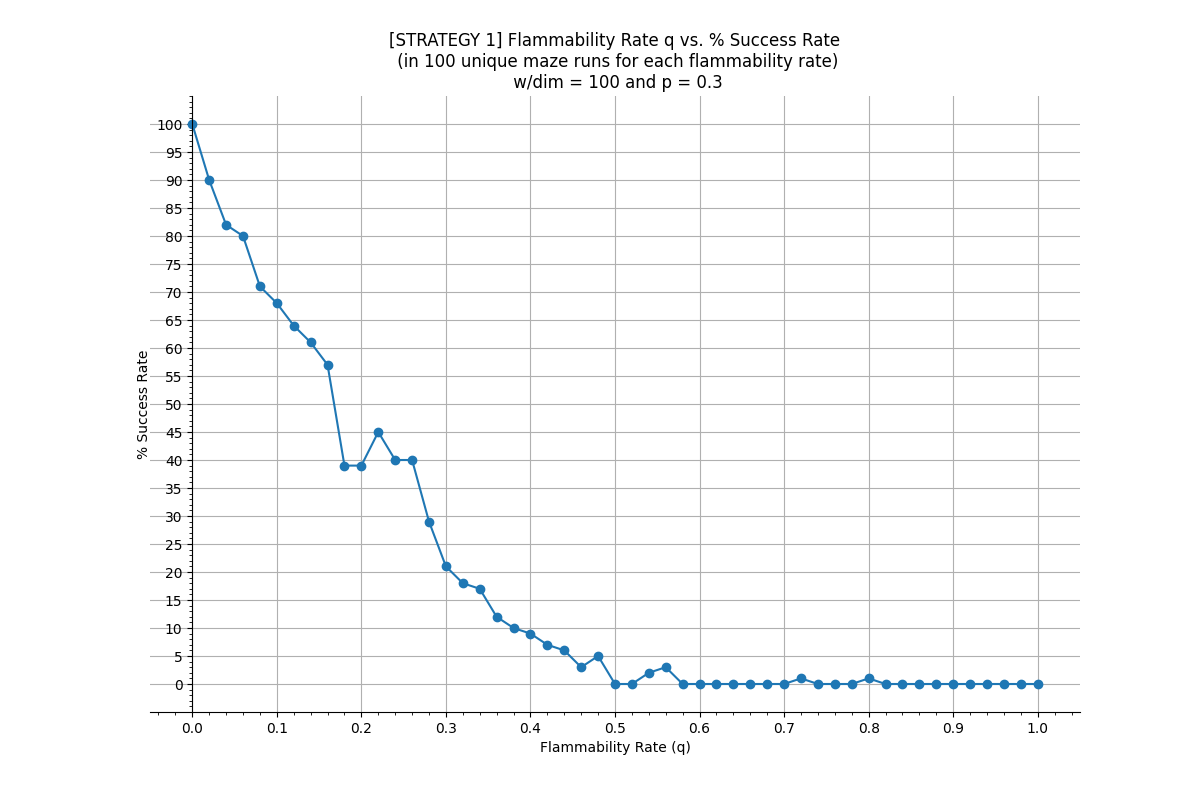
\includegraphics[scale=0.50]{Strategy1_q_successRate.PNG}
\caption{A graph of 'flammability rate q' vs 'strategy success rate' at $p = 0.3$ w/Strategy 1}
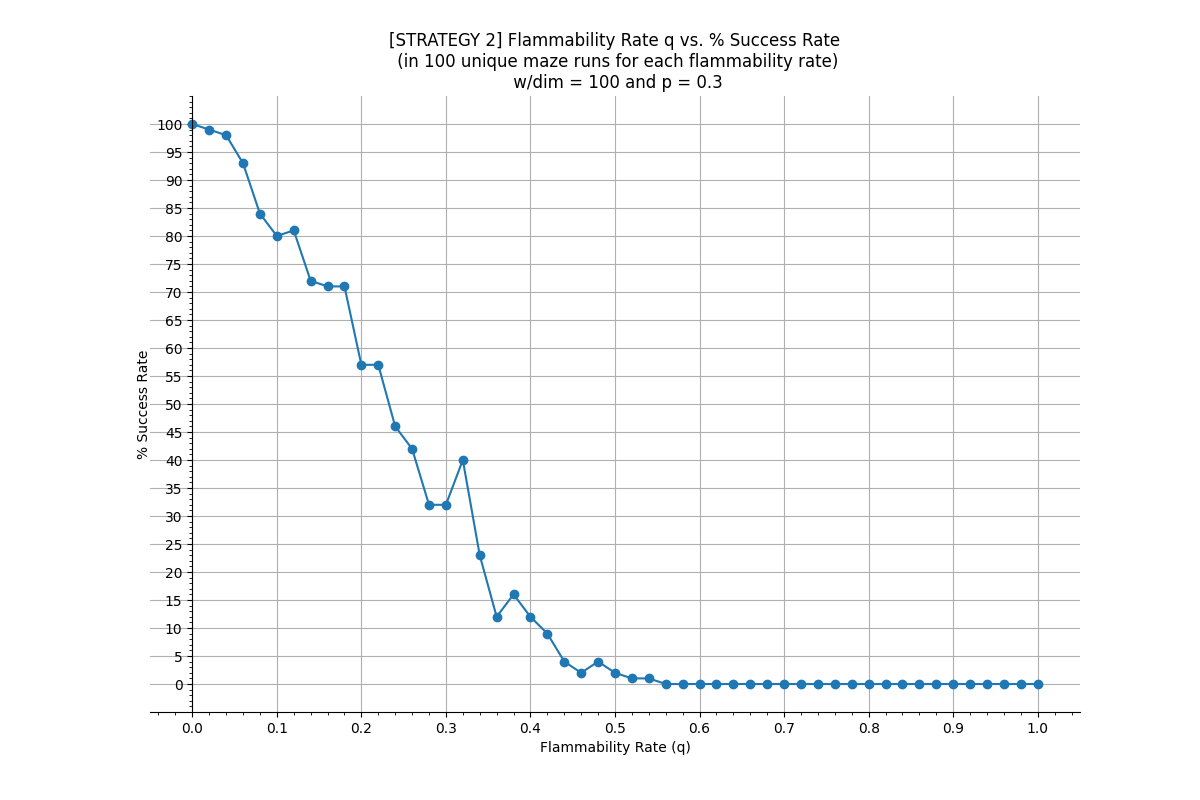
\includegraphics[scale=0.50]{Strategy2_q_successRate.PNG}
\caption{A graph of 'flammability rate q' vs 'strategy success rate' at $p = 0.3$ w/Strategy 2}
\end{figure}
\begin{figure}[!]
\centering
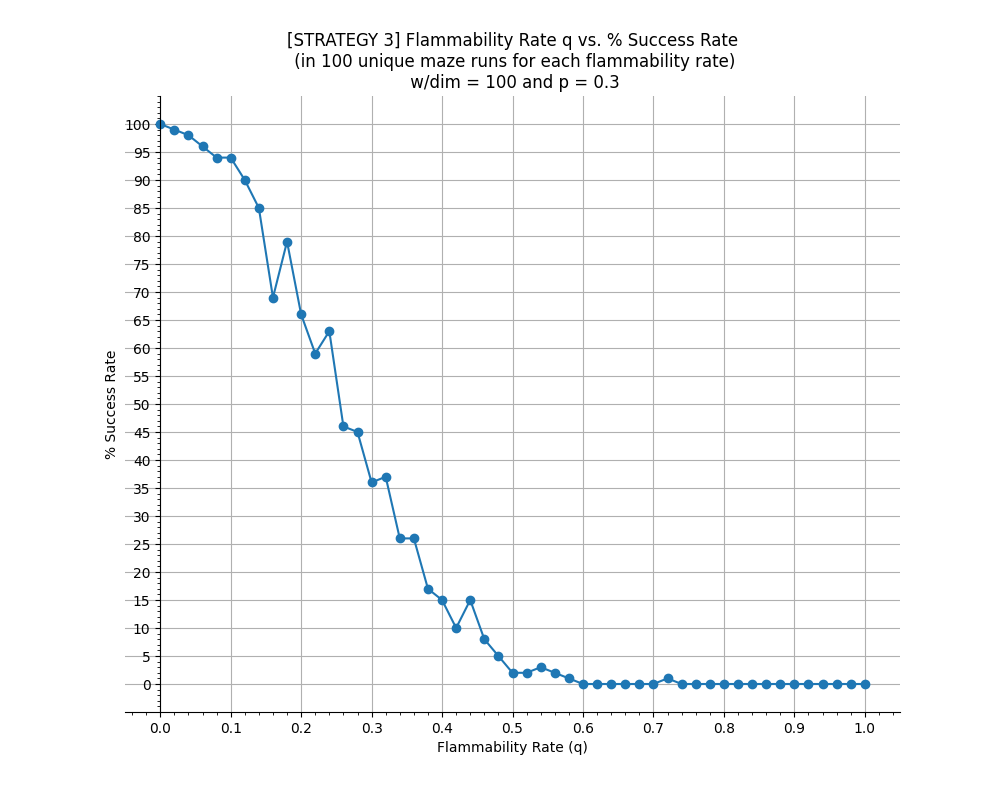
\includegraphics[scale=0.50]{Strategy3_q_successRate.PNG}
\caption{A graph of 'flammability rate q' vs 'strategy success rate' at $p = 0.3$ w/Strategy 3}
\end{figure}

All of these graphs have something in common: they all have a higher success rate with lower flammability rate than at higher probabilities. All of them, with the exception of luck and probability, seem to always fail with a probability of 0.6 or higher. From the looks of it, all of the data is focused on the left (anywhere before a flammability rate of 0.4). Our Strategy 3 seems to have a higher chance of success than the other two as it's curve is relatively high and doesn't fall down as quickly as Strategy 1 or 2. Both Strategy 2 and 3 seem to have a similar shape, and this may be because of how Strategy 3 was simply Strategy 2 but with a modified version of aStar as its main modification. Our Strategy 3 seemed to perform better overall despite having some questionable moves. Sure, it definitely has a better living chance than the other strategies because of the cost factor we created for it, but sometimes it would backtrack or go away from the goal space too much that the fire prevented it from entering in there, resulting in a loss. The cost factor helps it on the earlier ones as to not be engulfed in flames because it got too close, which was a common problem we have observed in testing both Strategy 1 and 2. As for the latter data, such as any flammability rate 0.6 or higher, it is really hard to say as our significant figures in measuring that data wouldn't let us see the potential each strategy had at that specific flammability rate. All that can really be said is that all of them have such minuscule chance of success that it's pretty much a failed run from the start. 
\pagebreak
\section{Theoretical Analysis: Unlimited Computational Power}
One limiting factor about theorizing and testing our algorithms were the computational powers of our devices. Simply put, there were times our devices can't handle the size of the fringes the algorithms needed, especially when it needed it for the bigger maze sizes, one massive example being BFS after exploring practically the entire maze. Another one was our ideas were limited based on what our devices could handle. As such, while we did think about a lot of fun ideas for this simulation, we weren't sure if our devices could handle it well. For instance, our implementation of aStarPlus felt weaker than what we originally thought about, despite having the ability to backtrack and a vision range of 3. It tended to avoid walls or deviate away from the goal unnecessarily because of how it was programmed.
One such thing we thought about for aStarPlus is actually having it create the path from the start to the goal, but also create multiple alternative paths should one be blocked off, as well as the cost of switching paths should it's current path be unavailable. This would make the agent have a finer looking path instead of what it is currently, and it would also prioritize the different paths based on how dangerous the paths are. For instance, if its current path is blocked off by a fire spreading and closing a gap, the agent would check the other paths and see which of the them were safer, which includes the cost to switch to the path, and take the path which had the minimum threats (which would simply be a priority queue). It would take up a lot of space because of the amount of paths it has to keep track of, but these paths can be removed once the path is deemed impossible for the agent by constantly checking its list of paths and seeing which path is valid. Sure, this will definitely increase the amount of time needed per move as well as the overall run time of aStarPlus, especially when it comes to bigger mazes, but it would be more consistent than it is currently.
\begin{verbatim}
#################################################################################
# Sample functions and added details of what we could've done, with pseudocode. #
#################################################################################

def pathValid(maze, path):
    if the path has any node assigned with 0 (obstacle) or 2 (fire)
        return false
    return true

in aStarPlus:
    pathsArr = [list of paths] # Stores all available paths here.
    pathsCost = [list of path's cost] # Stores path cost here, @same index.
    After moving, for all the paths in pathsArr:
        if pathValid(maze, pathsArr[i]) is false:
            pathsArr.pop(i)
        Update pathsArr[i] to make it follow the agent
    if current path is blocked or impossible:
        lowestCost = min(pathsCost)
        index = pathsCost.pop(lowestCost)
        newPath = pathsArr.pop(index)
        
Continue like normal, using newPath until it is no longer available\\
or it reaches the goal.
\end{verbatim}
The other fun idea we had was to make this more realistic. For instance, what if fires could go burn down on obstacle at a specific rate, or what if obstacles could be broken down by the agent by spending x amount of turns to break it down? What if the agent's vision range from aStarPlus was actually realistic and wasn't x-ray vision? These thoughts, plus various others, were intriguing ideas we had while working on our code. It would make our program run much slower, but it would be cool to witness and see how the agent would perform at least.
In general, if we had unlimited computational power, we would probably use it on improving the current aStarPlus and have it consider all possible paths to the goal based on its current position.
\section{There is No Time to Slack}
Currently, most of our search algorithms, aside from BFS, take only 1 second to find a path to the goal and reach it, with 1 second being it occurring most of the time, with the occasional 2 seconds based on probability. This is based on our current computational power with a maze size of around 500 x 500. It doesn't take more than 10 seconds to calculate each move, and if it did, it was from render.py having a sleepTime of a large number to visually comprehend the movements the agent made during the test.
Nonetheless, if we did only have 10 seconds to make a move, we would probably make it run based on gut reaction rather than simply calculating a path every single time. When we mean "gut reaction", we mean to simply check the agent's surrounding nodes and move towards the goal based on the dangers present. The more dangers, the more the agent will avoid it. It would be similar to our aStarPlus implementation and how it checks its nearby neighbors for the goal.
\section{Notable Information}
Crazy how 1 accidental OR instead of an AND can be the different between 2 seconds and 790 second :)
\end{document}